%        File: giddenStuCon.tex
%     Created: Thu Apr 12  9:00 AM 2011 C
% Last Change: Thu Apr 12 10:00 AM 2011 C
%    Based on: prelimPres.tex by Katy Huff
%\documentclass[11pt,handout]{beamer}
\documentclass[9pt]{beamer}
\usetheme[white]{Wisconsin}
%\title[short title]{long title}
\title[Cyclus Once-Through]{Cyclus Once-Through Fuel Cycle Benchmarks}
%\subtitle[short subtitle]{long subtitle}
\subtitle[VISION Comparisons]{Comparisons with VISION}
%\author[short name]{long name}
\author[M. Gidden]{Matthew J. Gidden}
%\date[short date]{long date}
\date[4.13.2012]{April 13, 2012}
%\institution[short name]{long name}
\institute[UW-Madison]{University of Wisconsin-Madison}
% Page numbers.
\setbeamertemplate{footline}[page number]
% Those icons  in the references are terrible looking.
\setbeamertemplate{bibliography item}[text]


\begin{document}
%%%%%%%%%%%%%%%%%%%%%%%%%%%%%%%%%%%%%%%%%%%%%%%%%%%%%%%%%%%%%
%% From uw-beamer Here's a handy bit of code to place at 
%% the beginning of your presentation (after \begin{document}):
\newcommand*{\alphabet}{ABCDEFGHIJKLMNOPQRSTUVWXYZabcdefghijklmnopqrstuvwxyz}
\newlength{\highlightheight}
\newlength{\highlightdepth}
\newlength{\highlightmargin}
\setlength{\highlightmargin}{2pt}
\settoheight{\highlightheight}{\alphabet}
\settodepth{\highlightdepth}{\alphabet}
\addtolength{\highlightheight}{\highlightmargin}
\addtolength{\highlightdepth}{\highlightmargin}
\addtolength{\highlightheight}{\highlightdepth}
\newcommand*{\Highlight}{\rlap{\textcolor{HighlightBackground}{\rule[-\highlightdepth]{\linewidth}{\highlightheight}}}}
%%%%%%%%%%%%%%%%%%%%%%%%%%%%%%%%%%%%%%%%%%%%%%%%%%%%%%%%%%%%%

%||||---------------
\frame{
\titlepage
}
%---------------||||


%||||---------------
\frame{
\frametitle{Outline}
\tableofcontents[]
}

%---------------||||
\section{Introduction}
% Overview : .tex
% put a repository model into cyclus
% that is capable of distinguishing between disposal choices
% and fuel cycle choices
% but is still speedy. 

\begin{frame}[ctb!]
  \frametitle{Introduction : Purpose}
  Fuel cycle simulators are designed to answer policy-related questions
  regarding transitions from one equilibrium state to another.

  \vspace{0.2cm}

  \pause
  A simulator answers the following questions as a function of its 
  parameter space:
  \begin{itemize}
    \item how much material exists
    \item where does that material reside
    \item from/to where and when is material transported
    \item what kinds of facilities are needed
    \item when is each type of facility needed
  \end{itemize}
\end{frame}

\begin{frame}[ctb!]
  \frametitle{Introduction : Cyclus}
  Cyclus is designed to provide a common fuel cycle simulator 
  framework.

  In this vein, we wish to show similar capabilities to other 
  simulators, e.g. VISION.

  This discussion will provide 
\end{frame}

\begin{frame}[ctb!]
  \frametitle{Introduction : VISION}
  VISION has surfaced as the industry standard simulator. It is well
  represented in the literature and can model most aspects of the
  fuel cycle. \cite{yacout_vision_2006}
  \begin{itemize}
    \item continuous material flows
    \item fleet-based facility deployment
    \item some regional modeling capability
    \item input/output via Excel
    \item simulation engine via Powersim
  \end{itemize}
  However, Powersim has its limitations...
  \begin{itemize}
    \item variables as a function of software level... did you get the academic or professional version?
    \item it's (relatively) expensive
    \item it's third party software
  \end{itemize}
\end{frame}

\section{Cyclus}
\subsection{Development}
\begin{frame}[ctb!]
  \frametitle{Development : From GENIUS to Cyclus}
  The predecessor of Cyclus was a simulator named GENIUSv2 \cite{oliver_geniusv2:_2009}
  \begin{itemize}
    \item also written in C++
    \item similar structures (regions - institutions - facilities)
    \item designed to overcome other simulator's difficulties
    \item not designed to proliferate a community
  \end{itemize}
\end{frame}

\begin{frame}[ctb!]
  \frametitle{Development : Developer Environment}
  Cyclus is designed to accommodate any kind of user or developer by
  allowing flexible participation \cite{huff_prelim_2011}
  \begin{figure}[htbp!]
    \begin{center}
      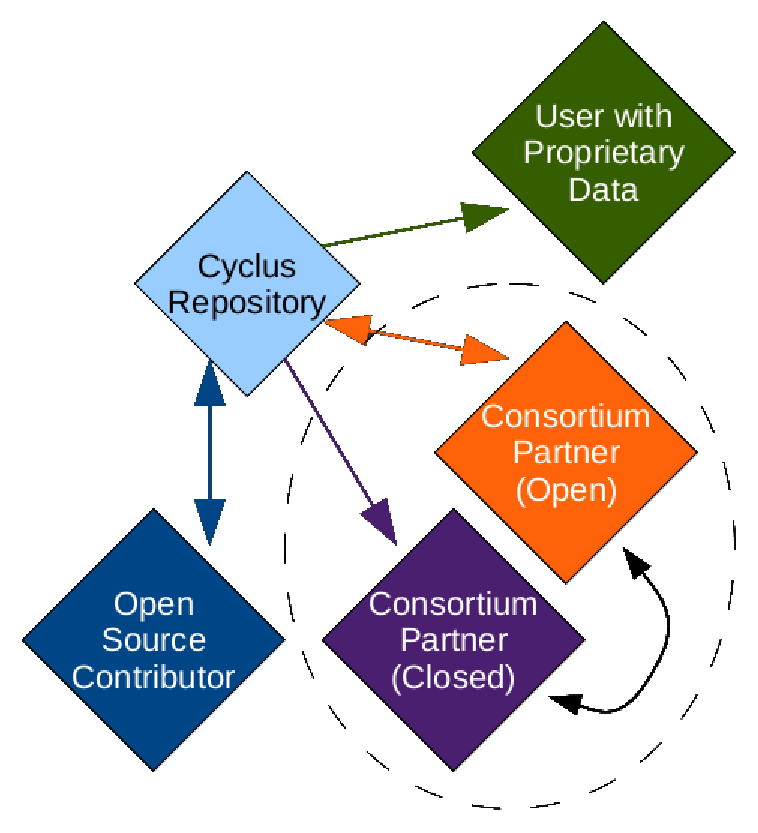
\includegraphics[height=4cm]{community.eps}
    \end{center}
    \caption{The Cyclus Participation Paradigm} 
    \label{fig:community}
  \end{figure}
\end{frame}

\begin{frame}[ctb!]
  \frametitle{Development : Code Repository}
  The Cyclus code repository is publicly available on GitHub.

  \vspace{0.2cm}

  General information can be found at cyclus.github.com.
  \begin{figure}[htbp!]
    \begin{center}
      \includegraphics[height=4cm]{cyclus-github.ps}
    \end{center}
    \caption{The Cyclus Github Landing Page} 
    \label{fig:cyclus-github}
  \end{figure}
\end{frame}

\begin{frame}[ctb!]
  \frametitle{Development : Code Repository}
  The Cyclus code repository is publicly available on GitHub.

  \vspace{0.2cm}

  The Cyclus source code can be found at github.com/cyclus/core.
  \begin{figure}[htbp!]
    \begin{center}
      \includegraphics[height=4cm]{github-core.ps}
    \end{center}
    \caption{The Cyclus Source Code Repository} 
    \label{fig:github-core}
  \end{figure}
\end{frame}

\begin{frame}[ctb!]
  \frametitle{Development : Model Modularity}
  Combined with the availability of the Cyclus engine source code,
  modularity of models in Cyclus plays a pivotal role in reducing its
  barriers to entry.

  \vspace{0.2cm}
  
  The Cyclus engine defines a Model's API, to which all models must
  conform. This allows models of each archetype to be interchangeable.
  \begin{figure}[htbp!]
    \begin{center}
      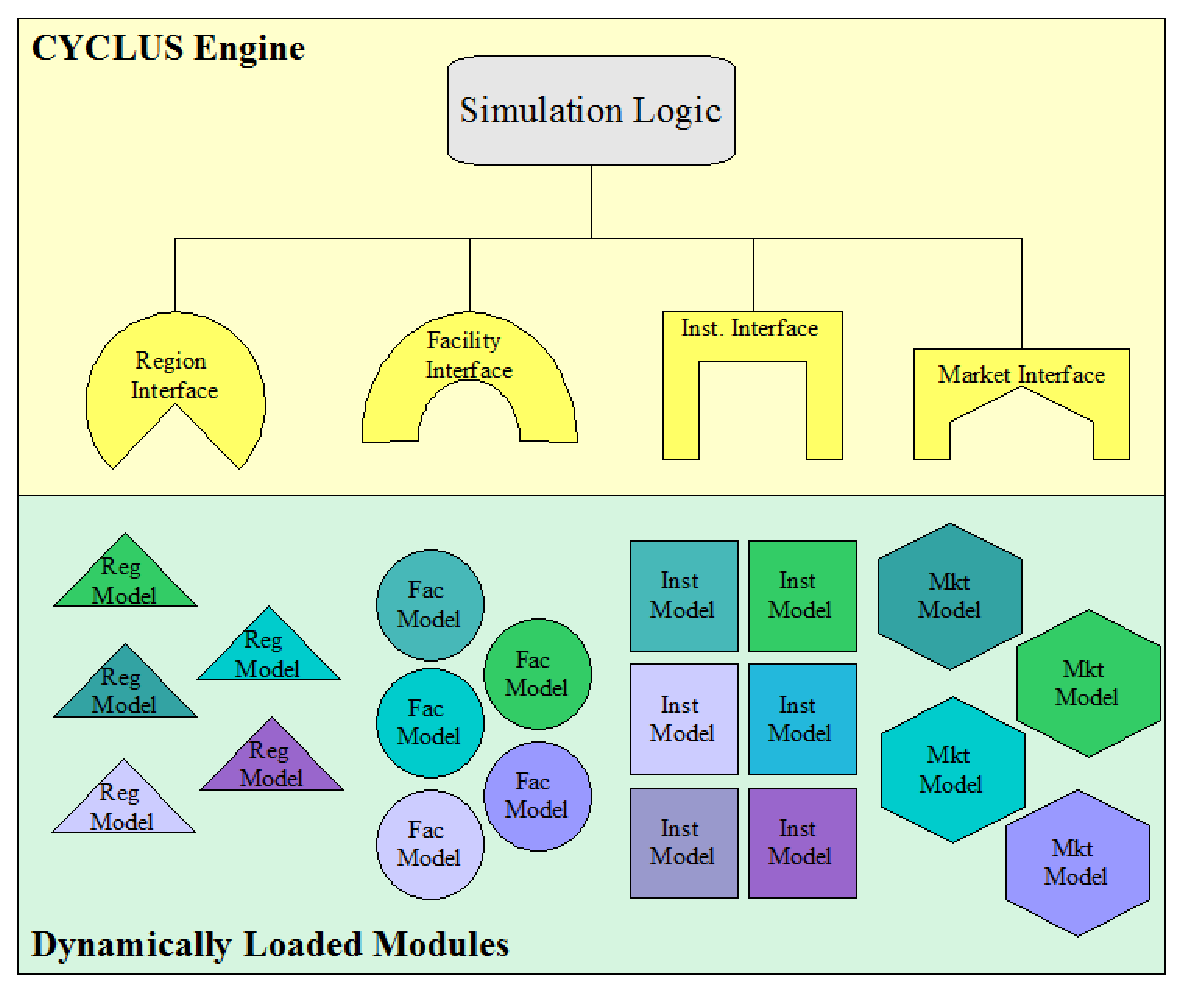
\includegraphics[height=5cm]{interfaces.eps}
    \end{center}
    \caption{Interface of Cyclus Models with the Engine} 
    \label{fig:interfaces}
  \end{figure}
\end{frame}

\subsection{Engine}
\begin{frame}[ctb!]
  \frametitle{Engine : Parent-Child Relationship and Time Steps}
  In the Cyclus Engine, Models communicate messages and commands through their 
  parent-child relationship.
  \begin{itemize}
    \item all models have parents
    \item all children are 'owned' by their parent
    \item the region-institution-facility relationship is modeled through this relationship
  \end{itemize}
  Simulation time steps are decomposed into:
  \begin{itemize}
    \item tick: system requirements determined
    \item resolve: optimized solution of requirements found
    \item tock: solution executed
  \end{itemize}
\end{frame}

\begin{frame}[ctb!]
  \frametitle{Engine : Black-Box Paradigm}
  Facilities are treated as black boxes, i.e. only what comes in and
  out is recorded.
  \begin{itemize}
    \item facilities can be thought of as nodes: sources, sinks, or intermediaries
    \item material is passed between resources as a combination of:
      \begin{itemize}
        \item commodities (e.g. fresh/spent fuel)
        \item recipes (e.g. 51 GWd/tHM burnup)
        \item quantity
      \end{itemize}
  \end{itemize}
  \begin{figure}[htbp!]
    \begin{center}
      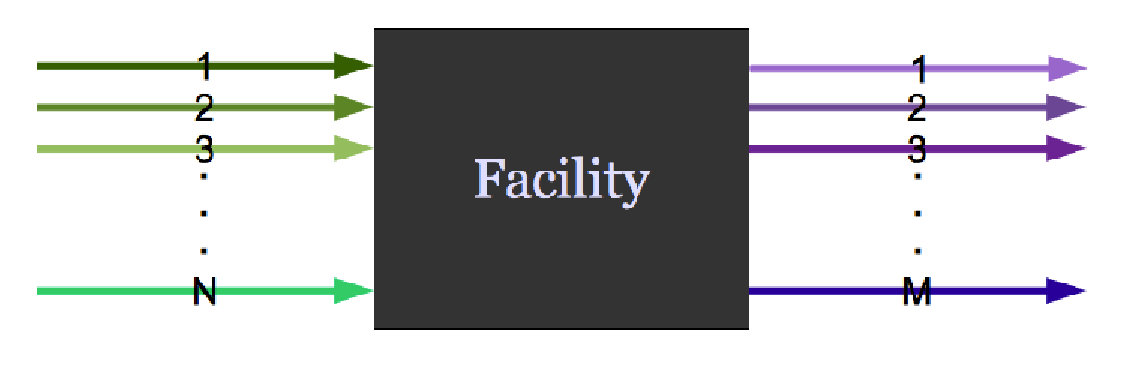
\includegraphics[height=3cm]{facility.eps}
    \end{center}
    \caption{Facilities are Black Boxes} 
    \label{fig:facility}
  \end{figure}
\end{frame}

\section{Benchmark Problems}
\begin{frame}[ctb!]
  \frametitle{Benchmarks : Overview}
  This suite of benchmark problems is designed to test Cyclus' build
  directive and gross material flows.
  
  \vspace {0.2cm}

  VISION is not a discrete material code, thus approximations must be made.
  As per Kyle Oliver's masters thesis, the following parameters are used:
  \begin{table}
  \centering
  \footnotesize{
    \begin{tabular}{|c|c|}
      \multicolumn{2}{c}{\textbf{Reactor Parameters for Benchmark Problems}}\\
      \hline
      Parameter                   & Value \\
      \hline
      Construction + License Time & 6 years \\
      Operation Time              & 60 years \\
      Power Capacity              & 1050 MWe \\
      Capacity Factor             & 0.9 \\ 
      Cycle Time                  & 12 months \\
      Burnup                      & 51 GWd/tHM \\
      Batches per Core            & 5 \\
      \hline
    \end{tabular}
    \caption[Reactor Parameters]{Full reactor parameters for the four benchmark problems}
    \label{tab:parameters}
  }
\end{table}

  
  \vspace {0.2cm}

  Note that using these parameters, a full core loading is 1.273 tHM.
\end{frame}

\begin{frame}[ctb!]
  \frametitle{Benchmarks : Specifics}
  Each simulation begins in the year 2000 and is run for 100 years. The decay 
  module in Cyclus has been turned off in order to compare results with given
  data.
  \begin{itemize}
    \item Problem 1 - 1 Reactor
      \begin{itemize}
        \item A single reactor is ordered in 2000, decommissioning at the end
          of its lifetime
      \end{itemize}
    \item Problem 2 - 10 Reactors
      \begin{itemize}
        \item 10 such reactors are ordered
      \end{itemize}
    \item Problem 3 - Linear Growth
      \begin{itemize}
        \item 1 reactor per year is built
        \item Note: 2 reactors are built in years that old reactors retire
      \end{itemize}
    %% \item Problem 4 - Exponential Growth
    %%   \begin{itemize}
    %%     \item Reactors are built in order to meet an increased electrical demand
    %%       of 2\% per year
    %%     \item Initial demand is 10 GWe
    %%     \item Initially, 10 legacy reactors exist
    %%     \item One legacy reactor per year is decommissioned starting in 2029
    %%   \end{itemize}
  \end{itemize}
\end{frame}


\section{Facility Modules}
\begin{frame}[ctb!]
  \frametitle{Facility Modules}
  Three types of facilities are used in the each benchmark:
  \begin{itemize}
    \item Source \& Sink Facilities
      \begin{itemize}
        \item Simple Facilities -- already existed
        \item Offer or request a certain amount of a commodity each time step
      \end{itemize}
    \item Batch Reactor Facility
      \begin{itemize}
        \item Developed for these benchmarks
        \item Beginning Phase: Requests a full core
        \item Operation Phase: Sits until cycle complete
        \item Refuel Phase: Ejects a batch and requests a batch
        \item Ending Phase: Ejects a full core
      \end{itemize}
  \end{itemize}
\end{frame}

\section{Results}
\begin{frame}[ctb!]
  \frametitle{Results : Problem 1}
  \begin{figure}[htbp!]
    \begin{center}
      \includegraphics[height=5cm]{p1.ps}
    \end{center}
    \caption{Problem 1 Results} 
    \label{fig:p1}
  \end{figure}
\end{frame}

\begin{frame}[ctb!]
  \frametitle{Results : Problem 2}
  \begin{figure}[htbp!]
    \begin{center}
      \includegraphics[height=5cm]{p2.ps}
    \end{center}
    \caption{Problem 2 Results} 
    \label{fig:p2}
  \end{figure}
\end{frame}

\begin{frame}[ctb!]
  \frametitle{Results : Problem 3}
  \begin{figure}[htbp!]
    \begin{center}
      \includegraphics[height=5cm]{p3.ps}
    \end{center}
    \caption{Problem 3 Results} 
    \label{fig:p3}
  \end{figure}
\end{frame}

%% \begin{frame}[ctb!]
%%   \frametitle{Results : Problem 4}
%%   \begin{figure}[htbp!]
%%     \begin{center}
%%       \includegraphics[height=5cm]{pichere.eps}
%%     \end{center}
%%     \caption{Problem 4 Results} 
%%     \label{fig:pichere}
%%   \end{figure}
%% \end{frame}

\begin{frame}[ctb!]
  \frametitle{Results : Future Work}
  \begin{itemize}
    \item ... lots?
    \item memory leaks \& efficient logging
    \item input/visualization team
    \item remaining VISION once-through benchmarks
    \item release 0.2!
  \end{itemize}
\end{frame}

\section{Acknowledgements}
\begin{frame}[ctb!]
  \frametitle{Acknowledgments}
  First and foremost, I would like to thank the members of the
  Computational Nuclear Engineering Research Group at UW 
  \begin{itemize}
    \item Katy Huff
    \item Robert Carlsen
    \item Prof. Paul Wilson
  \end{itemize}

  \vspace{0.2cm}

  And, of course, I would like to thank the DOE Office of Nuclear Energy's 
  Nuclear Engineering University Programs for providing funding. 
  \begin{figure}[htbp!]
    \begin{center}
      
\includegraphics[height=2cm]{neup.ps}
    \end{center}
    \label{fig:neup}
  \end{figure}
\end{frame}


%||||---------------
\begin{frame}%[allowframebreaks]
  \frametitle{References}
  \bibliographystyle{plain}
  \bibliography{giddenStuCon}
\end{frame}
%---------------||||




\end{document}
